\documentclass[]{iplresume} %Evil options: narrowline, wideline

%Font Info
\usepackage[T1]{fontenc}
\usepackage{graphicx}
\usepackage{float}
\usepackage{placeins}
\usepackage{hyperref}
\usepackage{breakurl}
\usepackage{url}

%Document Info
\title{機械学習アルゴリズムの分散グラフ処理フレームワークによる記述}
\author{Rathore Amogh}
\stdnum{1311216}
\office{岩崎研究室}
\lhead{電気通信大学 情報理工学部 情報・通信工学科 平成28年度卒業論文計画発表会}
\rhead{平成28年10月4日(金曜日)}

\begin{document}
\maketitle
\section{背景}
グラフはとてもフレキシブルな表現である。いろいろな分野のデータがグラフで表現できて、様々な問題が形式化ができる。今はビッグデータの時代で、量が大きいデータをグラフで表現すると非常にも大きいグラフになることが一般的である。そのような大きいグラフは一つの計算機で処理するのは無理である。なぜなら、一つの計算機はメモリが限られているし、プロセッサが一個なので、処理時間も長いからである。だから、グラフを分散して処理する必要がある。

分散グラフ処理はフレームワークがいくつか知られている。例えば、Apache GiraphやPregel+などのフレームワークがある。

近頃は、ビッグデータと同様に機械学習の分野も広がってきた。機械学習は人間が自然に行っている学習と同様の機能をコンピュータで実現する技術のことである。基本的には、機械学習がデータにパターンを見つけてデータについて学習を行うことである。ここもデータが大きいと処理時間が長くなるので、並列的に処理を行う必要がある。

\section{Vertex-centric approachによるグラフ処理}
Apache Giraph や Pregel+などはVertex-centric approachでグラフを処理するフレームワークである。Vertex-centric approach は各頂点が同じ関数を繰り替えして実行して、それでグラフ全体が処理されるアプローチのことである。GiraphとPregel+はスーパーステップという概念がある。一つのスーパーステップでグラフのすべての頂点がある同じ関数を一回実行して必要があったら他の頂点へメッセージを送る。受信側の頂点はそのメッセージを次のスーパーステップで受信する。

\section{目的と方針}
本研究では、機械学習のアルゴリズムを分散グラフ処理フレームワークで実装し、ライブラリ化を行う。さらに、性能の評価を行う。

まずは、グラフで表現できるアルゴリズムを幾つか探して、アルゴリズムの勉強を行う。次に、アルゴリズムで使うデータを集める。それから、Giraph での設計を考える。その設計に基づいて、アルゴリズムを実装して、実行してみる。次に、実装の一般化の設計を考えて、一般的な実装に変換する。そして、実行の性能を評価する。この方針で、様々のアルゴリズムを実装し、ライブラリ化を行って、性能を評価する。

\section{対象とする機械学習アルゴリズム}
実は機械学習のアルゴリズムには2種類あって、それは教師あり学習と教師なし学習のことである。本研究には、教師ありと教師なしを気にせずに、グラフで表現できるかどうかだけを気にして、アルゴリズムを選ぶことにする。今の段階では以下のアルゴリズムを対象とする。
\begin{itemize}
\item 人工ニューラルネットワーク(バックワードプロパゲーションアルゴリズム)
\item K平均法クラスタリング
\item 自己組織化写像
\end{itemize}

\section{人工ニューラルネットワーク}
人工ニューラルネットワークは、脳機能にみられるいくつかの特性を計算機上のシミュレーションによって表現することを目指した数学モデルである。図\ref{nn}から分かるように、ニューラルネットワークはレイヤーで分かれている。各レイヤーはニューロンがあって、ニューロンは次のレイヤーに辺を出している。一番目のレイヤーは入力レイヤーと呼ばれて、最後のレイヤーは出力レイヤーである。各ニューロンはアクティベートされるとき、何か計算をして、自分のアクティベーション値を求める。

\begin{figure}
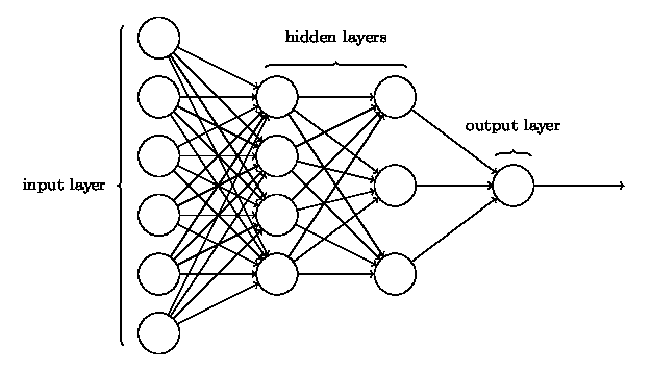
\includegraphics[scale=0.9]{nn.eps}
\caption{ニューラルネットワーク}
\label{nn}
\end{figure}

\section{バックワードプロパゲーションアルゴリズム}
教師あり機械学習はコスト関数という関数があって、それについてパラメータの最適化を行うことがよくある。バックワードプロパゲーションはニューラルネットワークでその最適化を行うアルゴリズムの一つである。このアルゴリズムは2段階で分かれている。1段階はフォワードプロパゲーションのことである。2段階はバックワードプロパゲーションである。
\begin{figure}
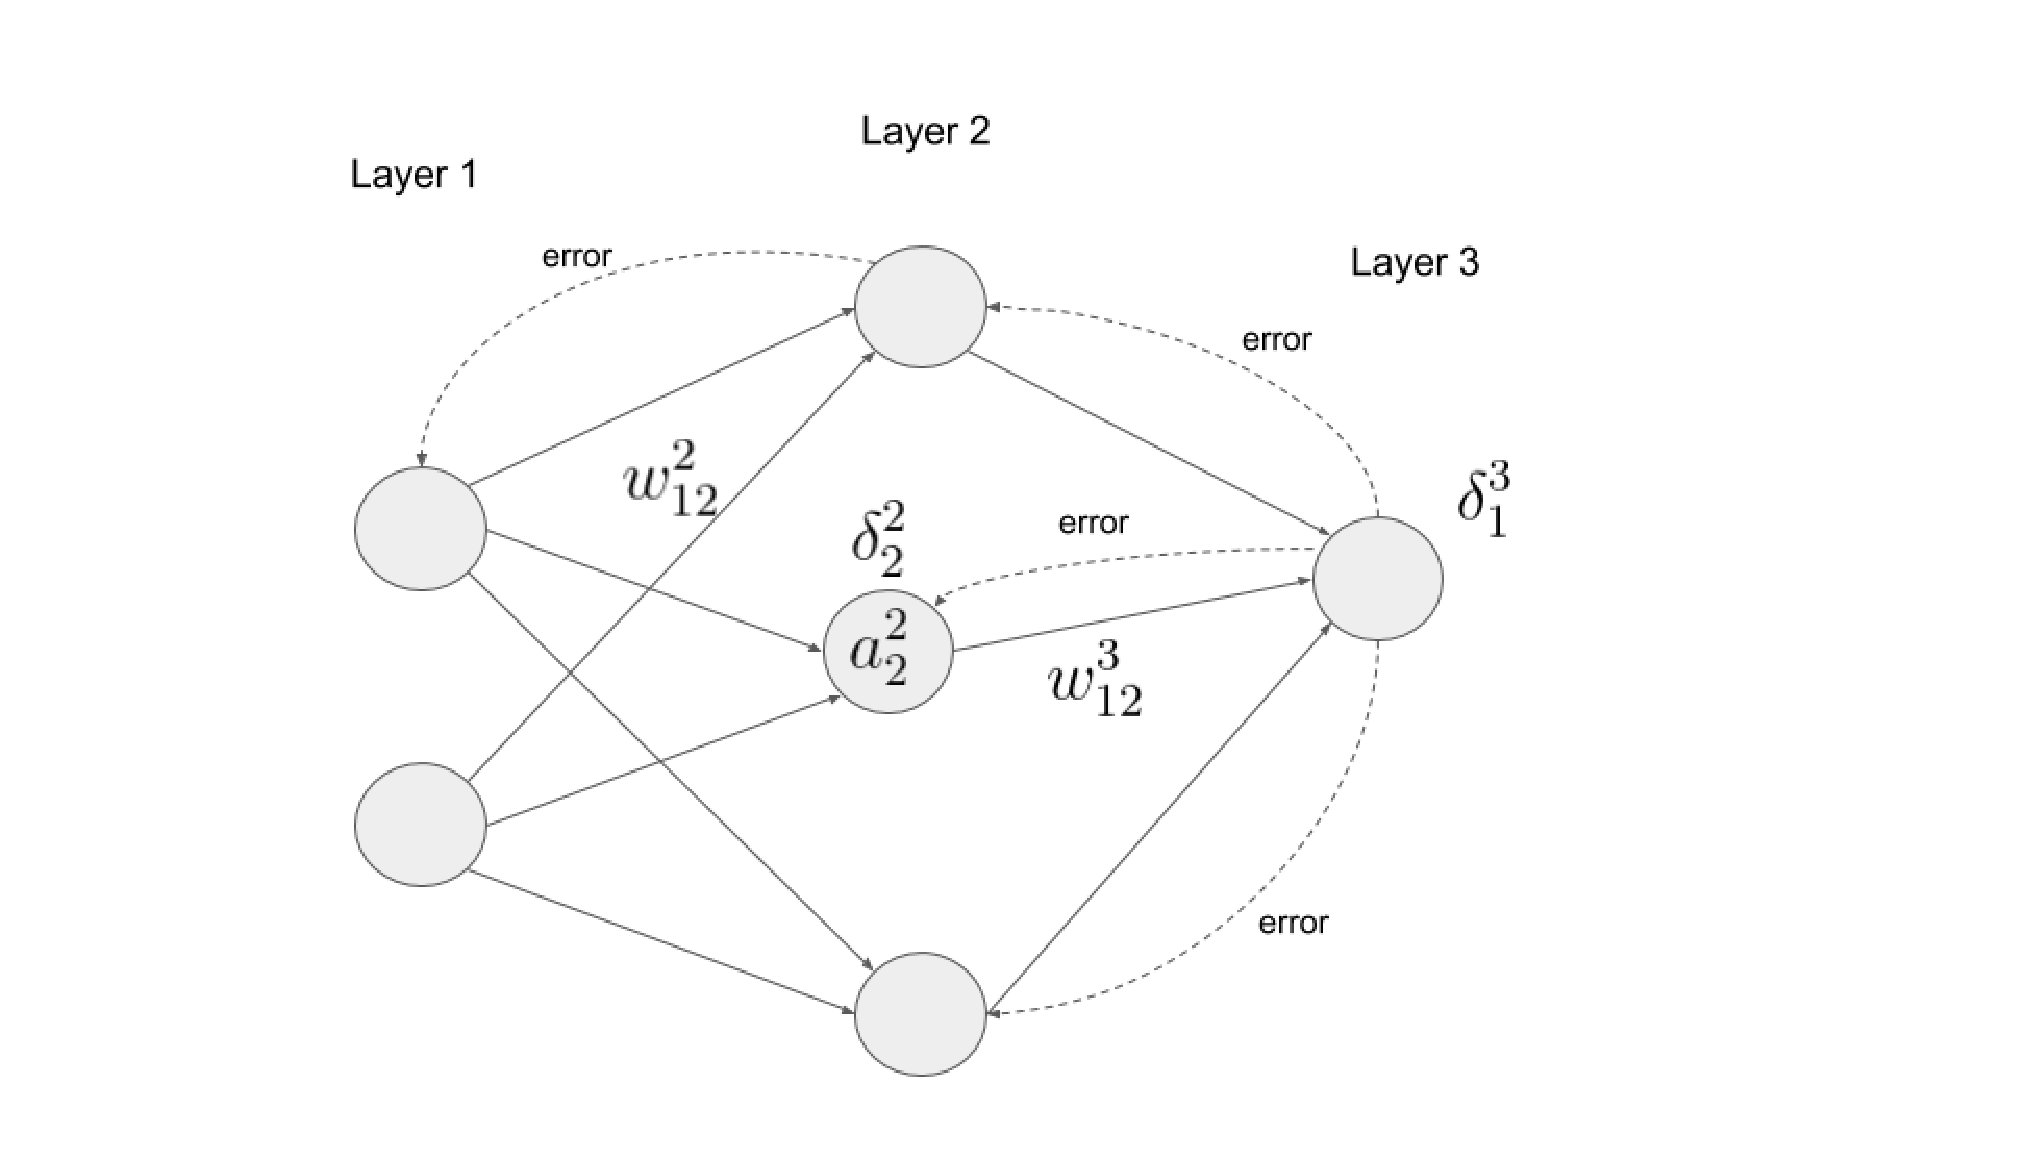
\includegraphics[scale=0.3]{backward.eps}
\caption{バックプロパゲーション}
\label{backward}
\end{figure}

図\ref{backward}から分かるように、各ニューロンと辺のウエイト(パラメータ)を$w^l_{jk}$と$a^l_j$で表すことがわかる。$w^l_{jk}$はレイヤー$l-1$のニューロン$k$からレイヤー$l$のニューロン$j$に行く辺のウエイト(パラメータ)の値である。$a^l_j$はレイヤー$l$のニューロン$j$のアクティベーションである。

フォワードプロパゲーションでは、各レイヤーのアクティベーションを、$a^l_j = S(\displaystyle\sum_k(w^l_{jk}a^{l-1}_k))$で計算する。ここで$S$はシグモイド関数である。入力レイヤーのアクティベーションは入力になるので、計算する必要がない。レイヤー2から出力レイヤーまですべてのレイヤーのアクティベーションを計算する。

フォワードプロパゲーションが終わったら、バックワードプロパゲーションで各ニューロンに付属されてるエラーを計算する。出力レイヤーのエラーは単にトレーニングデータの実際の出力マイナスニューラルネットワークが計算した出力結果の値とする。それで、出力レイヤーは自分のエラーを一個前のレイヤーにバックプロパゲート(渡す)する。前のレイヤーの$k$ニューロンのエラーを$\delta^l_k = \displaystyle\sum_j(w^{l+1}_{jk}\delta^{l+1}_j)S'(\displaystyle\sum_k(w^l_{jk}a^{l-1}_k))$で計算する。

フォワードとバックワードプロパゲーションが終わったら、Gradient Descentなどの最適化アルゴリズムによって、辺のウエイト(パラメータ)の値を更新して、また上のプロセスを繰り返す。

\section{Giraphでの実装の設計}
Giraphでバックワードプロパゲーションを実装するために、ニューロンを頂点、辺をグラフの辺にする。スーパーステップ1で入力レイヤーの各ニューロンがはレイヤー2のニューロンに自分のアクティベーション値を送る。スーパーステップ2では、レイヤー2のニューロンは自分のアクティベーションを計算して、結果をレイヤー3に渡す。これを繰り返して、出力レイヤーまでのアクティベーションをすべて計算する。このフォワードプロパゲーションには$L$スーパステップがかかる($L$はレイヤー数)。それから、前の節で述べた通り、各レイヤーはスーパステップ$L$からスーパーステップ$2L-1$でエラーをバックプロパゲートする。

これを一つのネットワークで行うと、$M$個トレーニングデータに対して$M$回同じ処理を行う必要がある。Giraphは並列処理フレームワークなので、$M$個データに対して$M$個のニューラルネットワークを作って、並列的にパラメータの最適化を行う。ここで、一個条件があって、それはすべてのニューラルネットワークの処理が終わるまでには、どのネットワークも先に次繰り返しを行うのはできないことである。なぜなら、すべてのネットワークはウエイトの値をシェアーするからである。一回の繰り返しが終わったら、ウエイトを更新するので、すべてのネットワークの処理結果によってウエイトを更新して、次の繰り返しを行う。

\section{まとめ}
上の節で述べた通り、機械学習の幾つかのアルゴリズムを分散グラフ処理フレームワークで実装して、アルゴリズムの実装とフレームワークの性能を評価する。さらに、実装のライブラリ化を行うことが本研究の目的である。対象とするフレームワークはまず Giraph で、時間があったらPregel+も含むようにする。

\section{現状と今後の予定}
機械学習の基本的なことを勉強を行った。特に、ニューラルネットワークについて調べて、バックワードプロパゲーションアルゴリズムの内容を理解した。そして、教師なし学習アルゴリズムのK平均法アルゴリズムの勉強を行った。さらに、分散グラフ処理フレームワークのGiraphとPregel+の構造を調べて、Giraphで最短経路問題を解くDijkstraのアルゴリズムを実装した。そして、ニューラルネットワークとバックワードプロパゲーションアルゴリズムのGiraphで実装する設計を少し考えた。

これから、バックワードプロパゲーションの設計をもっと具体的に考える。それから、バックワードプロパゲーションで解けられる機械学習問題を探して、それに対してニューラルネットワークをGiraphで実装する。次に、実装を一般化するための設計を考えて、実装の一般化を行う。同じことを他のアルゴリズムに対して繰り返す。

\begin{thebibliography}{9}
\bibitem{giraph}
Apache Giraph: \url{http://giraph.apache.org/}
\bibitem{Pregel Paper}
Pregel Paper: G. Malewicz et al., \textit{Pregel: A System for Large-Scale Graph Processing}, SIGMOD '10, ACM, 2010, pp. 135-146
\bibitem{pregel+}
Pregel$+$: \\
\url{http://www.cse.cuhk.edu.hk/pregelplus/download.html}
\bibitem{neural_net}
A Basic Introduction To Neural Networks \\
\url{http://pages.cs.wisc.edu/~bolo/shipyard/neural/local.html}
\bibitem{backprop}
Matt Mazur, \textit{A Step by Step Backpropagation Example} \\
\url{https://mattmazur.com/2015/03/17/a-step-by-step-backpropagation-example/}
\end{thebibliography}
\end{document}
